\documentclass[8pt,a4paper,compress]{beamer}

\usepackage{/home/siyer/lib/slides}
\usetikzlibrary{arrows,shapes,automata}
\usepackage{tabularx}

\newcolumntype{L}[1]{>{\raggedright\arraybackslash}p{#1}}
\newcolumntype{C}[1]{>{\centering\arraybackslash}p{#1}}
\newcolumntype{R}[1]{>{\raggedleft\arraybackslash}p{#1}}

\title{Lexical Analysis}
\date{}

\begin{document}
\begin{frame}
\vfill
\titlepage
\end{frame}

\section{Scanning Tokens}
\begin{frame}[fragile]
\pause

The first step in compiling a program is to break it into tokens (aka lexemes)

\pause\bigskip

Consider the \jmm program

\begin{tcolorbox}[enhanced,drop shadow southwest,sharp corners,size=fbox,colback=white,fontlower=\small\ttfamily,collower=silver900]

\begin{lstlisting}[language=Java,style=focusin]
package pass;

import java.lang.System;

public class Factorial {
    private static int n = 5;

    public static int factorial(int n) {
        if (n <= 0)
            return 1;
        else
            return n * factorial(n - 1);
    }
    
    public static void main(String[] args) {
        int x = n;
        System.out.println(x + "! = " + factorial(x));
    }
}
\end{lstlisting}

\tcblower
\begin{minipage}[t][.25cm][t]{\textwidth}
Factorial.java
\end{minipage}
\end{tcolorbox}

\pause

For \lstinline{Factorial.java}, we want to produce the sequence of tokens \lstinline{package}, \lstinline{pass}, \lstinline{;},\lstinline{import}, \lstinline{java}, \lstinline{.}, \lstinline{lang}, \lstinline{.}, \lstinline{System},\lstinline{;}, \lstinline{public}, \lstinline{class}, \lstinline{Factorial}, \lstinline${$, and so on
\end{frame}

\begin{frame}[fragile]
\pause

We separate the lexemes into categories

\pause\bigskip

In \lstinline{Factorial.java}
\begin{itemize}
\pause
\item \lstinline{public}, \lstinline{class}, \lstinline{static}, and \lstinline{void} are reserved words

\pause
\item \lstinline{Factorial}, \lstinline{main}, \lstinline{String}, \lstinline{args}, \lstinline{System}, \lstinline{out}, and \lstinline{println} are all identifiers

\pause
\item The token \lstinline{"!="} is a literal, a string literal in this instance

\pause
\item The rest are operators and separators
\end{itemize}

\pause\bigskip

The program that breaks the source program into a sequence of tokens is called a lexical analyzer or a scanner

\pause\bigskip

A scanner may be hand-crafted or it may be generated from a specification consisting of regular expressions
\end{frame}

\begin{frame}[fragile]
\pause

State transition diagrams can be used for describing scanners

\pause\bigskip

A state transition diagram for recognizing identifiers and integers

\begin{center}
\begin{tikzpicture}[>=stealth',shorten >=1pt,auto,node distance=2cm,initial text=]
  \node[initial,state] (0) at (0, 0)  {start};
  \node[state] (1) at (2, 1) {id};
  \node[state] (2) at (2, -1) {int};
  \node[state,accepting] (3) at (4, 1) {idEnd};
  \node[state,accepting] (4) at (4, -1) {intEnd};
  \path[->] (0)  edge node             {\lstinline{letter, _, $}} (1);
  \path[->] (0)  edge node             {\lstinline{1...9}} (2);  
  \path[->] (0)  edge [bend right=100,below] node             {\lstinline{0}} (4);    
  \path[->] (1)  edge [loop above] node             {\lstinline{letter, digit, _, $}} (1);    
  \path[->] (2)  edge [loop below] node             {\lstinline{digit}} (2);      
  \path[->] (1)  edge node {} (3);    
  \path[->] (2)  edge node {} (4);    
\end{tikzpicture}
\end{center}
\end{frame}

\begin{frame}[fragile]
\pause

\begin{overprint}
\onslide<2|handout:1>
\begin{tcolorbox}[enhanced,drop shadow southwest,sharp corners,size=fbox,colback=white,fontlower=\small\ttfamily,collower=silver900]

\begin{lstlisting}[language=Java,style=focusin]
    if (isLetter(ch) || ch == '_' || ch == '$') {
        buffer = new StringBuffer();
        while (isLetter(ch) || isDigit(ch) || 
               ch == '_' || ch == '$') {
            buffer.append(ch);
            nextCh();
        }
        return new TokenInfo(IDENTIFIER, buffer.toString(), line);
    }
    else if (ch == '0') {
        nextCh();
        return new TokenInfo(INT_LITERAL, "0", line);
    }
    else if (isDigit(ch)){
        buffer = new StringBuffer();
        while (isDigit(ch)) {
            buffer.append(ch);
            nextCh();
        }
        return new TokenInfo(INT_LITERAL, buffer.toString(), line);
    }
\end{lstlisting}

\tcblower
\begin{minipage}[t][.25cm][t]{\textwidth}
scanning identifiers and integers
\end{minipage}
\end{tcolorbox}

\onslide<3|handout:2>
\begin{tcolorbox}[enhanced,drop shadow southwest,sharp corners,size=fbox,colback=white,fontlower=\small\ttfamily,collower=silver900]

\begin{lstlisting}[language=Java,style=focusin,backgroundcolor=\color{lime100}]
    if (isLetter(ch) || ch == '_' || ch == '$') {
        buffer = new StringBuffer();
        while (isLetter(ch) || isDigit(ch) || 
               ch == '_' || ch == '$') {
            buffer.append(ch);
            nextCh();
        }
        return new TokenInfo(IDENTIFIER, buffer.toString(), line);
    }
\end{lstlisting}
\begin{lstlisting}[language=Java,style=focusout]
    else if (ch == '0') {
        nextCh();
        return new TokenInfo(INT_LITERAL, "0", line);
    }
    else if (isDigit(ch)){
        buffer = new StringBuffer();
        while (isDigit(ch)) {
            buffer.append(ch);
            nextCh();
        }
        return new TokenInfo(INT_LITERAL, buffer.toString(), line);
    }
\end{lstlisting}

\tcblower
\begin{minipage}[t][.25cm][t]{\textwidth}
scan and return an identifier
\end{minipage}
\end{tcolorbox}

\onslide<4|handout:3>
\begin{tcolorbox}[enhanced,drop shadow southwest,sharp corners,size=fbox,colback=white,fontlower=\small\ttfamily,collower=silver900]

\begin{lstlisting}[language=Java,style=focusout]
    if (isLetter(ch) || ch == '_' || ch == '$') {
        buffer = new StringBuffer();
        while (isLetter(ch) || isDigit(ch) || 
               ch == '_' || ch == '$') {
            buffer.append(ch);
            nextCh();
        }
        return new TokenInfo(IDENTIFIER, buffer.toString(), line);
    }
\end{lstlisting}
\begin{lstlisting}[language=Java,style=focusin,backgroundcolor=\color{lime100}]
    else if (ch == '0') {
        nextCh();
        return new TokenInfo(INT_LITERAL, "0", line);
    }
\end{lstlisting}
\begin{lstlisting}[language=Java,style=focusout]
    else if (isDigit(ch)){
        buffer = new StringBuffer();
        while (isDigit(ch)) {
            buffer.append(ch);
            nextCh();
        }
        return new TokenInfo(INT_LITERAL, buffer.toString(), line);
    }
\end{lstlisting}

\tcblower
\begin{minipage}[t][.25cm][t]{\textwidth}
scan and return the integer 0
\end{minipage}
\end{tcolorbox}

\onslide<5|handout:4>
\begin{tcolorbox}[enhanced,drop shadow southwest,sharp corners,size=fbox,colback=white,fontlower=\small\ttfamily,collower=silver900]

\begin{lstlisting}[language=Java,style=focusout]
    if (isLetter(ch) || ch == '_' || ch == '$') {
        buffer = new StringBuffer();
        while (isLetter(ch) || isDigit(ch) || 
               ch == '_' || ch == '$') {
            buffer.append(ch);
            nextCh();
        }
        return new TokenInfo(IDENTIFIER, buffer.toString(), line);
    }
    else if (ch == '0') {
        nextCh();
        return new TokenInfo(INT_LITERAL, "0", line);
    }
\end{lstlisting}
\begin{lstlisting}[language=Java,style=focusin,backgroundcolor=\color{lime100}]
    else if (isDigit(ch)){
        buffer = new StringBuffer();
        while (isDigit(ch)) {
            buffer.append(ch);
            nextCh();
        }
        return new TokenInfo(INT_LITERAL, buffer.toString(), line);
    }
\end{lstlisting}

\tcblower
\begin{minipage}[t][.25cm][t]{\textwidth}
scan and return an integer different from 0
\end{minipage}
\end{tcolorbox}
\end{overprint}
\end{frame}

\begin{frame}[fragile]
\pause

A state transition diagram for recognizing keywords

\begin{center}
\begin{tikzpicture}[>=stealth',shorten >=1pt,auto,node distance=2cm,initial text=]
  \node[initial,state] (0) at (0, 0)  {start};
  \node[state] (1) at (2.5, 0) {id};
  \node[state,accepting] (2) at (4.5, 0) {idEnd};
  \node[] (3) at (7, 1.2) {keyword};
  \node[] (4) at (7, -1.2) {identifier};
  \path[->] (0)  edge node             {\lstinline{letter, _, $}} (1);
  \path[->] (1)  edge [loop above] node             {\lstinline{letter, digit, _, $}} (1);    
  \path[->] (1)  edge node {} (2);    
  \path[->] (2)  edge node {\lstinline{reserved}} (3);    
  \path[->] (2)  edge node {\lstinline{!reserved}} (4);      
\end{tikzpicture}
\end{center}
\end{frame}

\begin{frame}[fragile]
\pause

\onslide<2->
\begin{tcolorbox}[enhanced,drop shadow southwest,sharp corners,size=fbox,colback=white,fontlower=\small\ttfamily,collower=silver900]

\begin{lstlisting}[language=Java,style=focusin]
reserved = new Hashtable<String, Integer>();
reserved.put("abstract", ABSTRACT);  
reserved.put("boolean", BOOLEAN);         
reserved.put("char", CHAR);
...
reserved.put("while", WHILE);
\end{lstlisting}

\tcblower
\begin{minipage}[t][.25cm][t]{\textwidth}
table of reserved words
\end{minipage}
\end{tcolorbox}

\bigskip

\begin{overprint}
\onslide<3|handout:1>
\begin{tcolorbox}[enhanced,drop shadow southwest,sharp corners,size=fbox,colback=white,fontlower=\small\ttfamily,collower=silver900]

\begin{lstlisting}[language=Java,style=focusin]
    if (isLetter(ch) || ch == '_' || ch == '$') {
        buffer = new StringBuffer();
        while (isLetter(ch) || isDigit(ch) || 
               ch == '_' || ch == '$'){
            buffer.append(ch);
            nextCh();
        }
        String identifier = buffer.toString();                 
        if (reserved.containsKey(identifier)) {
            return new TokenInfo(reserved.get(identifier), line); 
        }
        else {                     
            return new TokenInfo(IDENTIFIER, identifier, line);                 
        }
    }
\end{lstlisting}

\tcblower
\begin{minipage}[t][.25cm][t]{\textwidth}
scanning keywords
\end{minipage}
\end{tcolorbox}

\onslide<4|handout:2>
\begin{tcolorbox}[enhanced,drop shadow southwest,sharp corners,size=fbox,colback=white,fontlower=\small\ttfamily,collower=silver900]

\begin{lstlisting}[language=Java,style=focusout]
    if (isLetter(ch) || ch == '_' || ch == '$') {
\end{lstlisting}
\begin{lstlisting}[language=Java,style=focusin,backgroundcolor=\color{lime100}]
        buffer = new StringBuffer();
        while (isLetter(ch) || isDigit(ch) || 
               ch == '_' || ch == '$'){
            buffer.append(ch);
            nextCh();
        }
        String identifier = buffer.toString();                 
\end{lstlisting}
\begin{lstlisting}[language=Java,style=focusout]
        if (reserved.containsKey(identifier)) {
            return new TokenInfo(reserved.get(identifier), line); 
        }
        else {                     
            return new TokenInfo(IDENTIFIER, identifier, line);                 
        }
    }
\end{lstlisting}

\tcblower
\begin{minipage}[t][.25cm][t]{\textwidth}
scan an identifier
\end{minipage}
\end{tcolorbox}

\onslide<5|handout:3>
\begin{tcolorbox}[enhanced,drop shadow southwest,sharp corners,size=fbox,colback=white,fontlower=\small\ttfamily,collower=silver900]

\begin{lstlisting}[language=Java,style=focusout]
    if (isLetter(ch) || ch == '_' || ch == '$') {
        buffer = new StringBuffer();
        while (isLetter(ch) || isDigit(ch) || 
               ch == '_' || ch == '$'){
            buffer.append(ch);
            nextCh();
        }
        String identifier = buffer.toString();                 
\end{lstlisting}
\begin{lstlisting}[language=Java,style=focusin,backgroundcolor=\color{lime100}]
        if (reserved.containsKey(identifier)) {
            return new TokenInfo(reserved.get(identifier), line); 
        }
\end{lstlisting}
\begin{lstlisting}[language=Java,style=focusout]
        else {                     
            return new TokenInfo(IDENTIFIER, identifier, line);                 
        }
    }
\end{lstlisting}

\tcblower
\begin{minipage}[t][.25cm][t]{\textwidth}
return as keyword if identifier is reserved
\end{minipage}
\end{tcolorbox}

\onslide<6|handout:4>
\begin{tcolorbox}[enhanced,drop shadow southwest,sharp corners,size=fbox,colback=white,fontlower=\small\ttfamily,collower=silver900]

\begin{lstlisting}[language=Java,style=focusout]
    if (isLetter(ch) || ch == '_' || ch == '$') {
        buffer = new StringBuffer();
        while (isLetter(ch) || isDigit(ch) || 
               ch == '_' || ch == '$'){
            buffer.append(ch);
            nextCh();
        }
        String identifier = buffer.toString();                 
        if (reserved.containsKey(identifier)) {
            return new TokenInfo(reserved.get(identifier), line); 
        }
\end{lstlisting}
\begin{lstlisting}[language=Java,style=focusin,backgroundcolor=\color{lime100}]
        else {                     
            return new TokenInfo(IDENTIFIER, identifier, line);                 
        }
\end{lstlisting}
\begin{lstlisting}[language=Java,style=focusout]
    }
\end{lstlisting}

\tcblower
\begin{minipage}[t][.25cm][t]{\textwidth}
return as identifier otherwise
\end{minipage}
\end{tcolorbox}
\end{overprint}
\end{frame}

\begin{frame}[fragile]
\pause

A state transition diagram for recognizing separators and operators

\begin{center}
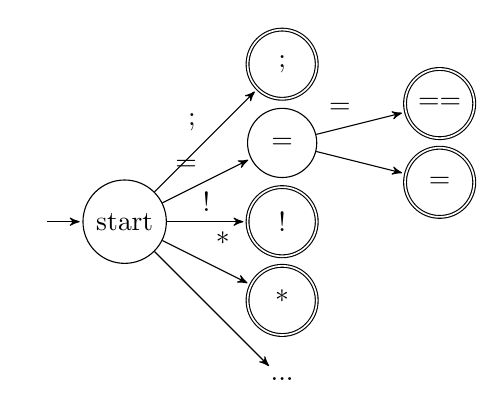
\begin{tikzpicture}[>=stealth',shorten >=1pt,auto,node distance=2cm,initial text=]
  \node[initial,state] (0) at (0, 0)  {start};
  \node[state,accepting] (1) at (2, 0) {\lstinline{!}};
  \node[state] (2) at (2, 1) {\lstinline{=}};
  \node[state,accepting] (3) at (2, 2) {\lstinline{;}};  
  \node[state,accepting] (4) at (2, -1) {\lstinline{*}};  
  \node[] (5) at (2, -2) {\lstinline{...}};  
  \node[state,accepting] (6) at (4, 1.5) {\lstinline{==}};
  \node[state,accepting] (7) at (4, .5) {\lstinline{=}};
  \path[->] (0)  edge node             {\lstinline{!}} (1);  
  \path[->] (0)  edge node             {\lstinline{=}} (2);    
  \path[->] (0)  edge node             {\lstinline{;}} (3);    
  \path[->] (0)  edge node             {\lstinline{*}} (4);    
  \path[->] (0)  edge node             {} (5);    
  \path[->] (2)  edge node             {\lstinline{=}} (6);    
  \path[->] (2)  edge node             {} (7);    
\end{tikzpicture}
\end{center}
\end{frame}

\begin{frame}[fragile]
\pause

\begin{overprint}
\onslide<2|handout:1>
\begin{tcolorbox}[enhanced,drop shadow southwest,sharp corners,size=fbox,colback=white,fontlower=\small\ttfamily,collower=silver900]

\begin{lstlisting}[language=Java,style=focusin]
switch (ch) {
...
case ';':
    nextCh();             
    return new TokenInfo(SEMI, line);         
case '=':             
    nextCh();             
    if (ch == '=') {                 
        nextCh();                 
        return new TokenInfo(EQUAL, line);             
    }             
    else {                 
        return new TokenInfo(ASSIGN, line);             
    }         
case '!':             
    nextCh();             
    return new TokenInfo(LNOT, line);         
case '*':             
    nextCh();             
    return new TokenInfo(STAR, line);
...
}
\end{lstlisting}

\tcblower
\begin{minipage}[t][.25cm][t]{\textwidth}
scanning separators and operators
\end{minipage}
\end{tcolorbox}

\onslide<3|handout:2>
\begin{tcolorbox}[enhanced,drop shadow southwest,sharp corners,size=fbox,colback=white,fontlower=\small\ttfamily,collower=silver900]

\begin{lstlisting}[language=Java,style=focusout]
switch (ch) {
...
\end{lstlisting}
\begin{lstlisting}[language=Java,style=focusin,backgroundcolor=\color{lime100}]
case ';':
    nextCh();             
    return new TokenInfo(SEMI, line);         
\end{lstlisting}
\begin{lstlisting}[language=Java,style=focusout]
case '=':             
    nextCh();             
    if (ch == '=') {                 
        nextCh();                 
        return new TokenInfo(EQUAL, line);             
    }             
    else {                 
        return new TokenInfo(ASSIGN, line);             
    }         
case '!':             
    nextCh();             
    return new TokenInfo(LNOT, line);         
case '*':             
    nextCh();             
    return new TokenInfo(STAR, line);
...
}
\end{lstlisting}

\tcblower
\begin{minipage}[t][.25cm][t]{\textwidth}
scan and return ;
\end{minipage}
\end{tcolorbox}

\onslide<4|handout:3>
\begin{tcolorbox}[enhanced,drop shadow southwest,sharp corners,size=fbox,colback=white,fontlower=\small\ttfamily,collower=silver900]

\begin{lstlisting}[language=Java,style=focusout]
switch (ch) {
...
case ';':
    nextCh();             
    return new TokenInfo(SEMI, line);         
\end{lstlisting}
\begin{lstlisting}[language=Java,style=focusin,backgroundcolor=\color{lime100}]
case '=':             
    nextCh();             
    if (ch == '=') {                 
        nextCh();                 
        return new TokenInfo(EQUAL, line);             
    }             
    else {                 
        return new TokenInfo(ASSIGN, line);             
    }         
\end{lstlisting}
\begin{lstlisting}[language=Java,style=focusout]
case '!':             
    nextCh();             
    return new TokenInfo(LNOT, line);         
case '*':             
    nextCh();             
    return new TokenInfo(STAR, line);
...
}
\end{lstlisting}

\tcblower
\begin{minipage}[t][.25cm][t]{\textwidth}
scan and return == or =
\end{minipage}
\end{tcolorbox}

\onslide<5|handout:4>
\begin{tcolorbox}[enhanced,drop shadow southwest,sharp corners,size=fbox,colback=white,fontlower=\small\ttfamily,collower=silver900]

\begin{lstlisting}[language=Java,style=focusout]
switch (ch) {
...
case ';':
    nextCh();             
    return new TokenInfo(SEMI, line);         
case '=':             
    nextCh();             
    if (ch == '=') {                 
        nextCh();                 
        return new TokenInfo(EQUAL, line);             
    }             
    else {                 
        return new TokenInfo(ASSIGN, line);             
    }         
\end{lstlisting}
\begin{lstlisting}[language=Java,style=focusin,backgroundcolor=\color{lime100}]
case '!':             
    nextCh();             
    return new TokenInfo(LNOT, line);         
\end{lstlisting}
\begin{lstlisting}[language=Java,style=focusout]
case '*':             
    nextCh();             
    return new TokenInfo(STAR, line);
...
}
\end{lstlisting}

\tcblower
\begin{minipage}[t][.25cm][t]{\textwidth}
scan and return !
\end{minipage}
\end{tcolorbox}

\onslide<6|handout:5>
\begin{tcolorbox}[enhanced,drop shadow southwest,sharp corners,size=fbox,colback=white,fontlower=\small\ttfamily,collower=silver900]

\begin{lstlisting}[language=Java,style=focusout]
switch (ch) {
...
case ';':
    nextCh();             
    return new TokenInfo(SEMI, line);         
case '=':             
    nextCh();             
    if (ch == '=') {                 
        nextCh();                 
        return new TokenInfo(EQUAL, line);             
    }             
    else {                 
        return new TokenInfo(ASSIGN, line);             
    }         
case '!':             
    nextCh();             
    return new TokenInfo(LNOT, line);         
\end{lstlisting}
\begin{lstlisting}[language=Java,style=focusin,backgroundcolor=\color{lime100}]
case '*':             
    nextCh();             
    return new TokenInfo(STAR, line);
\end{lstlisting}
\begin{lstlisting}[language=Java,style=focusout]
...
}
\end{lstlisting}

\tcblower
\begin{minipage}[t][.25cm][t]{\textwidth}
scan and return *
\end{minipage}
\end{tcolorbox}

\end{overprint}
\end{frame}

\begin{frame}[fragile]
\pause

A state transition diagram for recognizing whitespace

\begin{center}
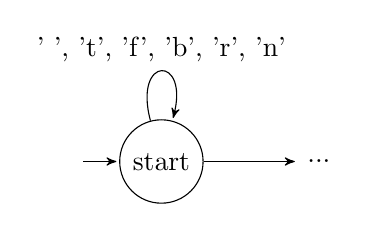
\begin{tikzpicture}[>=stealth',shorten >=1pt,auto,node distance=2cm,initial text=]
  \node[initial,state] (0) at (0, 0)  {start};
  \node[] (1) at (2, 0) {\lstinline{...}};  
  \path[->] (0)  edge [loop above] node             {\lstinline{' ', '\\t', '\\f', '\\b', '\\r', '\\n'}} (0);  
  \path[->] (0)  edge node             {} (1);    
\end{tikzpicture}
\end{center}

\pause\bigskip

\begin{tcolorbox}[enhanced,drop shadow southwest,sharp corners,size=fbox,colback=white,fontlower=\small\ttfamily,collower=silver900]

\begin{lstlisting}[language=Java,style=focusin]
while (isWhitespace(ch)) {                 
    nextCh();             
}
\end{lstlisting}

\tcblower
\begin{minipage}[t][.25cm][t]{\textwidth}
scanning whitespace
\end{minipage}
\end{tcolorbox}
\end{frame}

\begin{frame}[fragile]
\pause

A state transition diagram for recognizing comments

\begin{center}
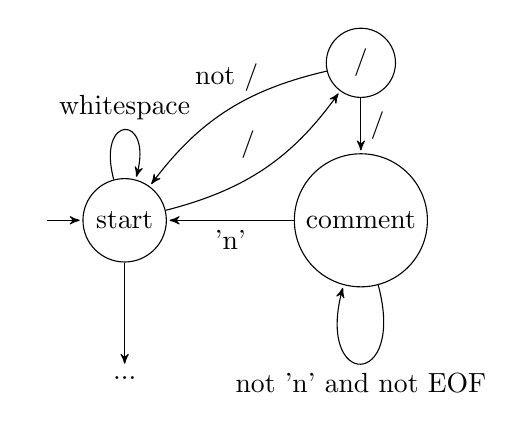
\begin{tikzpicture}[>=stealth',shorten >=1pt,auto,node distance=2cm,initial text=]
  \node[initial,state] (0) at (0, 0)  {start};
  \node[state] (1) at (3, 0) {comment};  
  \node[state] (2) at (3, 2) {\lstinline{/}};    
  \node[] (3) at (0, -2) {\lstinline{...}};      
  \path[->] (0)  edge [loop above] node             {whitespace} (0);  
  \path[->] (2)  edge[bend left=-20,above,inner sep=7] node             {not \lstinline{/}} (0);      
  \path[->] (0)  edge[bend right=20] node             {\lstinline{/}} (2);    
  \path[->] (2)  edge node             {\lstinline{/}} (1);      
  \path[->] (1)  edge node             {\lstinline{'\\n'}} (0);        
  \path[->] (1)  edge[loop below] node {not \lstinline{'\\n'} and not \lstinline{EOF}} (1);
  \path[->] (0)  edge node             {} (3);          
\end{tikzpicture}
\end{center}
\end{frame}

\begin{frame}[fragile]
\pause

\begin{overprint}
\onslide<2|handout:1>
\begin{tcolorbox}[enhanced,drop shadow southwest,sharp corners,size=fbox,colback=white,fontlower=\small\ttfamily,collower=silver900]

\begin{lstlisting}[language=Java,style=focusin]
boolean moreWhiteSpace = true;
while (moreWhiteSpace) {
    while (isWhitespace(ch)) {
        nextCh();
    }
    if (ch == '/') {
        nextCh();
        if (ch == '/') { 
            while (ch != '\n' && ch != EOFCH) {
                nextCh();
            }
        }
        else {
            reportScannerError(
                "Operator / is not supported in j--.");
        }
    }
    else {
        moreWhiteSpace = false;
    }
}
\end{lstlisting}

\tcblower
\begin{minipage}[t][.25cm][t]{\textwidth}
scanning comments
\end{minipage}
\end{tcolorbox}

\onslide<3|handout:2>
\begin{tcolorbox}[enhanced,drop shadow southwest,sharp corners,size=fbox,colback=white,fontlower=\small\ttfamily,collower=silver900]

\begin{lstlisting}[language=Java,style=focusout]
boolean moreWhiteSpace = true;
while (moreWhiteSpace) {
    while (isWhitespace(ch)) {
        nextCh();
    }
    if (ch == '/') {
        nextCh();
\end{lstlisting}
\begin{lstlisting}[language=Java,style=focusin,backgroundcolor=\color{lime100}]
        if (ch == '/') { 
            while (ch != '\n' && ch != EOFCH) {
                nextCh();
            }
        }
\end{lstlisting}
\begin{lstlisting}[language=Java,style=focusout]
        else {
            reportScannerError(
                "Operator / is not supported in j--.");
        }
    }
    else {
        moreWhiteSpace = false;
    }
}
\end{lstlisting}

\tcblower
\begin{minipage}[t][.25cm][t]{\textwidth}
scan and ignore comments
\end{minipage}
\end{tcolorbox}

\onslide<4|handout:3>
\begin{tcolorbox}[enhanced,drop shadow southwest,sharp corners,size=fbox,colback=white,fontlower=\small\ttfamily,collower=silver900]

\begin{lstlisting}[language=Java,style=focusout]
boolean moreWhiteSpace = true;
while (moreWhiteSpace) {
    while (isWhitespace(ch)) {
        nextCh();
    }
    if (ch == '/') {
        nextCh();
        if (ch == '/') { 
            while (ch != '\n' && ch != EOFCH) {
                nextCh();
            }
        }
\end{lstlisting}
\begin{lstlisting}[language=Java,style=focusin,backgroundcolor=\color{lime100}]
        else {
            reportScannerError(
                "Operator / is not supported in j--.");
        }
\end{lstlisting}
\begin{lstlisting}[language=Java,style=focusout]
    }
    else {
        moreWhiteSpace = false;
    }
}
\end{lstlisting}

\tcblower
\begin{minipage}[t][.25cm][t]{\textwidth}
error!
\end{minipage}
\end{tcolorbox}
\end{overprint}
\end{frame}

\section{Regular Expressions}
\begin{frame}[fragile]
\pause

Regular expressions provide a notation for describing patterns of characters in a text

\pause\bigskip

A regular expression desbribes a language of strings over an alphabet $\Sigma$

\pause\bigskip

$\epsilon$ (epsilon) describes the language consisting of only the empty string

\pause\bigskip
If $a \in \Sigma$, then $a$ describes the language $L(a)$ consisting of the string $a$

\pause\bigskip
If $r$ and $s$ are regular expressions, then their concatenation $rs$ describes the language $L(rs)$ consisting of all strings obtained by concatenating a string from $L(r)$ to a string from $L(s)$

\pause\bigskip
If $r$ and $s$ are regular expressions, then their alternation $r|s$ describes the language $L(r|s)$ consisting of all strings from $L(r)$ or $L(s)$

\pause\bigskip
If $r$ is a regular expression, then the repetition (aka the Kleene closure) $r*$ describes the language $L(r*)$ consisting of all strings obtained by concatenating zero or more instances of strings from $L(r)$

\pause\bigskip
Both $r$ and $(r)$ describe the same language, ie, $L(r) = L((r))$
\end{frame}

\begin{frame}[fragile]
\pause

For example, given an alphabet $\Sigma = \{a,b\}$

\begin{itemize}
\pause
\item $a(a|b)*$ describes the language of \pause non-empty strings of $a$'s and $b$'s, beginning with an $a$

\pause
\item $aa | ab | ba | bb$ describes the language of \pause all two-symbol strings over the alphabet

\pause
\item $(a|b)\!*\!ab$ describes the language of \pause all strings of $a$'s and $b$'s, ending in $ab$
\end{itemize}

\pause\bigskip

In a programming language such as Java
\begin{itemize}
\pause
\item Reserved words may be described as \lstinline{abstract | boolean | char | ... | while}

\pause
\item Operators may be described as \lstinline{= | == | > | ... | *}

\pause
\item Identifiers may be described as \lstinline{([a-zA-Z] | _ | $)([a-zA-Z0-9] | _ | $)*}
\end{itemize}
\end{frame}

\section{Finite State Automata}
\begin{frame}[fragile]
\pause

For any language described by a regular expression, there is a state transition diagram called Finite State Automaton that can recognize strings in the language

\pause\bigskip

A Finite State Automaton (FSA) $F$ is a quintuple $F = (\Sigma, S, s_0, F, M)$, where
\begin{enumerate}
\pause
\item $\Sigma$ is the input alphabet

\pause
\item $S$ is a set of states

\pause
\item $s_0 \in S$ is a special start state

\pause
\item $F \in S$ is a set of final states

\pause
\item $M$ is a set of moves or state transitions of the form $m(r, a) = s$, where $r,s \in S$ and $a \in \Sigma$
\end{enumerate}
\end{frame}

\begin{frame}[fragile]
\pause

For example, consider the regular expression $(a|b)a\!*\!b$ over the alphabet $\{a, b\}$

\pause\bigskip

An FSA $F$ that recognizes the language described by the regular expression

\begin{center}
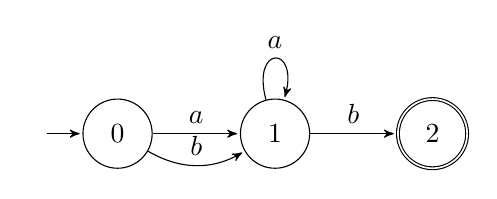
\begin{tikzpicture}[>=stealth',shorten >=1pt,auto,node distance=2cm,initial text=]
  \node[initial,state]   (0) at (0, 0)  {0};
  \node[state]           (1) at (2, 0)  {1};
  \node[state,accepting] (2) at (4, 0)  {2};
  \path[->] (0)  edge node             {$a$} (1);
  \path[->] (0)  edge[bend right] node {$b$} (1);
  \path[->] (1)  edge[loop above] node {$a$} (1);
  \path[->] (1)  edge node             {$b$} (2);
\end{tikzpicture}
\end{center}

\pause\bigskip
Formally, $F = (\Sigma, S, s_0, F, M)$, where $\Sigma = \{a, b\}$, $S = \{0, 1, 2\}$, $s_0 = 0$, $F = \{2\}$, and $M$ is
\begin{center}
\begin{tabular}{|c|c|c|} \hline
$r$ & $a$ & $m(r, a)$ \\ \hline \hline
$0$ & $a$ & $1$ \\ \hline
$0$ & $b$ & $1$ \\ \hline
$1$ & $a$ & $1$ \\ \hline
$1$ & $b$ & $2$ \\ \hline
\end{tabular}
\end{center}
\end{frame}

\section{Non-deterministic (NFA) Versus Deterministic Finite State Automata (DFA)}
\begin{frame}[fragile]
\pause

A non-deterministic finite state automaton (NFA) is one that allows
\begin{itemize}
\pause
\item An $\epsilon$-move defined on the empty string $\epsilon$, ie, $m(r, \epsilon) = s$

\pause
\item More than one move from the same state on the same input symbol $a$, ie, $m(r, a) = s$ and $m(r, a) = t$, \noindent where $s \neq t$
\end{itemize}

\pause\bigskip

An NFA is said to recognize an input string if, starting in the start state, there exists a set of moves based on the input that takes us into one of the final states

\pause\bigskip

A deterministic finite state automaton (DFA) is one without $\epsilon$-moves, and there is a unique move from any state on an input symbol $a$, ie, if $m(r, a) = s$ and $m(r, a) = t$, then $s = t$
\end{frame}

\begin{frame}[fragile]
\pause

For example, consider the regular expression $a(a|b)\!*\!b$ over the alphabet $\{a, b\}$

\pause\bigskip

An NFA $N$ that recognizes the language described by the regular expression

\begin{center}
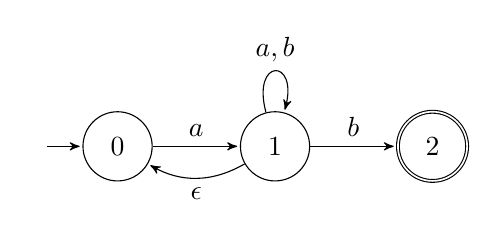
\begin{tikzpicture}[>=stealth',shorten >=1pt,auto,node distance=2cm,initial text=]
  \node[initial,state]   (0) at (0, 0)  {0};
  \node[state]           (1) at (2, 0)  {1};
  \node[state,accepting] (2) at (4, 0)  {2};
  \path[->] (0)  edge node             {$a$} (1);
  \path[->] (1)  edge[bend left] node {$\epsilon$} (0);
  \path[->] (1)  edge[loop above] node {$a, b$} (1);
  \path[->] (1)  edge node             {$b$} (2);
\end{tikzpicture}
\end{center}

\pause\bigskip

Formally, $N = (\Sigma, S, s_0, F, M)$ where $\Sigma = \{a, b\}$, $S = \{0, 1, 2\}$, $s_0 = 0$, $F = \{2\}$, and $M$ is
\begin{center}
\begin{tabular}{|c|c|c|} \hline
$r$ & $a$ & $m(r, a)$ \\ \hline \hline
$0$ & $a$ & $1$ \\ \hline
$1$ & $\epsilon$ & $0$ \\ \hline
$1$ & $a$ & $1$ \\ \hline
$1$ & $b$ & $1$ \\ \hline
$1$ & $b$ & $2$ \\ \hline
\end{tabular}
\end{center}
\end{frame}

\section{Regular Expressions to NFA}
\begin{frame}[fragile]
\pause

Given any regular expression $r$, we can construct (using Thompson's construction procedure) an NFA $N$ that recognizes the same language; ie, $L(N) = L(r)$

\pause\bigskip

(Rule 1) NFA $N_r$ for recognizing $L(r = \epsilon)$

\begin{center}
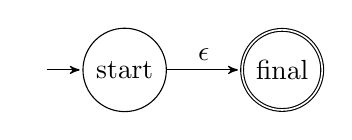
\begin{tikzpicture}[>=stealth',shorten >=1pt,auto,node distance=2cm,initial text=]
  \node[initial,state]   (0) at (0, 0) {start};
  \node[state,accepting] (1) at (2, 0) {final};
  \path[->] (0)  edge node             {$\epsilon$} (1);
\end{tikzpicture}
\end{center}

\pause\bigskip

(Rule 2) NFA $N_r$ for recognizing $L(r = a)$

\begin{center}
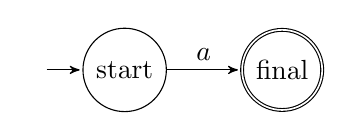
\begin{tikzpicture}[>=stealth',shorten >=1pt,auto,node distance=2cm,initial text=]
  \node[initial,state]   (0) at (0, 0) {start};
  \node[state,accepting] (1) at (2, 0) {final};
  \path[->] (0)  edge node             {$a$} (1);
\end{tikzpicture}
\end{center}
\end{frame}

\begin{frame}[fragile]
\pause\bigskip

(Rule 3) NFA $N_{rs}$ for recognizing $L(rs)$

\begin{center}
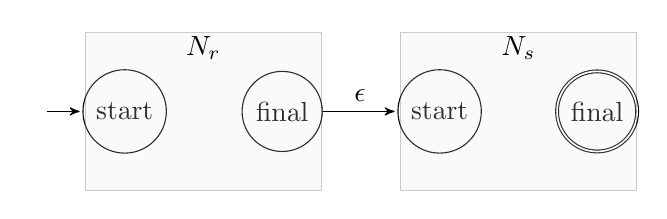
\begin{tikzpicture}[>=stealth',shorten >=1pt,auto,node distance=2cm,initial text=]
  \node[initial,state]   (0) at (0, 0)              {start};
  \node[state]           (1) at (2, 0)  {final};
  \node[state]           (2) at (4, 0)  {start};
  \node[state,accepting] (3) at (6, 0)  {final};
  \path[->] (1)  edge node             {$\epsilon$} (2);  
  \path[draw=black,fill=black!10,opacity=0.2] (-.5,-1) -- (-.5,1) -- (2.5,1) -- (2.5,-1) -- cycle; 
  \node[] at (1, 0.8) {$N_r$};
  \path[draw=black,fill=black!10,opacity=0.2] (3.5,-1) -- (3.5,1) -- (6.5,1) -- (6.5,-1) -- cycle; 
  \node[] at (5, 0.8) {$N_s$};
\end{tikzpicture}
\end{center}

\pause\bigskip

(Rule 4) NFA $N_{r|s}$ for recognizing $L(r|s)$

\begin{center}
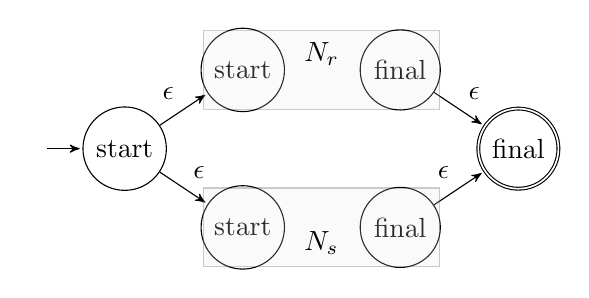
\begin{tikzpicture}[>=stealth',shorten >=1pt,auto,node distance=2cm,initial text=]
  \node[initial,state] (0) at (0, 0)  {start};
  \node[state] (1) at (1.5, 1) {start};
  \node[state] (2) at (1.5, -1) {start};  
  \node[state] (3) at (3.5, 1) {final};
  \node[state] (4) at (3.5, -1) {final};  
  \node[state,accepting] (5) at (5, 0) {final};
  \path[->] (0)  edge node             {$\epsilon$} (1);
  \path[->] (0)  edge node             {$\epsilon$} (2);
  \path[->] (3)  edge node             {$\epsilon$} (5);
  \path[->] (4)  edge node             {$\epsilon$} (5);
  \path[draw=black,fill=black!10,opacity=0.2] (1,.5) -- (1,1.5) -- (4,1.5) -- (4,.5) -- cycle; 
  \node[] at (2.5, 1.2) {$N_r$};
  \path[draw=black,fill=black!10,opacity=0.2] (1,-1.5) -- (1,-.5) -- (4,-.5) -- (4,-1.5) -- cycle; 
  \node[] at (2.5, -1.2) {$N_s$};
\end{tikzpicture}
\end{center}
\end{frame}

\begin{frame}[fragile]
\pause

(Rule 5) NFA $N_{r*}$ for recognizing $L(r*)$

\begin{center}
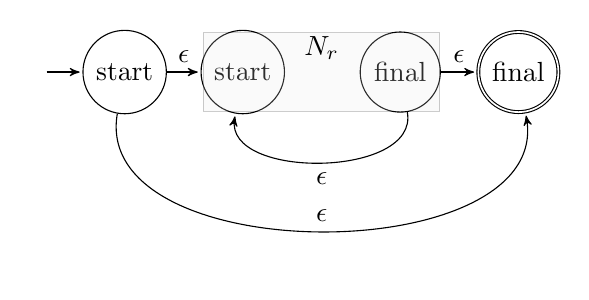
\begin{tikzpicture}[>=stealth',shorten >=1pt,auto,node distance=2cm,initial text=]
  \node[initial,state] (0) at (0, 0)  {start};
  \node[state] (1) at (1.5, 0) {start};
  \node[state] (2) at (3.5, 0) {final};
  \node[state,accepting] (3) at (5, 0) {final};
  \path[->] (0)  edge node             {$\epsilon$} (1);
  \path[->] (2)  edge node             {$\epsilon$} (3);
  \path[->] (2)  edge [bend left=100] node {$\epsilon$} (1);
  \path[->] (0)  edge [bend right=100] node {$\epsilon$} (3);
  \path[draw=black,fill=black!10,opacity=0.2] (1,-.5) -- (1,.5) -- (4,.5) -- (4,-.5) -- cycle; 
  \node[] at (2.5, .3) {$N_r$};
\end{tikzpicture}
\end{center}

\pause\bigskip

(Rule 6) NFA $N_r$ for recognizing $L(r)$ also recognizes $L((r))$
\end{frame}

\begin{frame}[fragile]
\pause

As an example, let's construct an NFA for the regular expression $(a|b)a\!*\!b$, proceeding from left to right

\pause\bigskip

Using Rule 2, we get the NFAs $N_a$ and $N_b$ for recognizing $a$ and $b$ as

\pause

\begin{center}
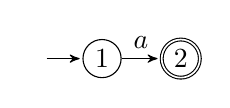
\begin{tikzpicture}[>=stealth',shorten >=1pt,auto,node distance=2cm,initial text=]
  \tikzset{every state/.style={inner sep=2pt,minimum size=0pt}}
  \node[initial,state]   (1) at (0, 0) {1};
  \node[state,accepting] (2) at (1, 0) {2};
  \path[->] (1)  edge node             {$a$} (2);
\end{tikzpicture}
\end{center}

\pause

\begin{center}
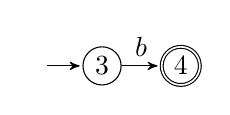
\begin{tikzpicture}[>=stealth',shorten >=1pt,auto,node distance=2cm,initial text=]
  \tikzset{every state/.style={inner sep=2pt,minimum size=0pt}}
  \node[initial,state]   (3) at (0, 0) {3};
  \node[state,accepting] (4) at (1, 0) {4};
  \path[->] (3)  edge node             {$b$} (4);
\end{tikzpicture}
\end{center}

\pause\smallskip

Using Rules 4 and 6, we get the NFA $N_{(a|b)}$ for recognizing $(a|b)$ as

\pause

\begin{center}
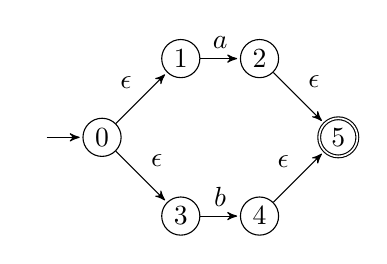
\begin{tikzpicture}[>=stealth',shorten >=1pt,auto,node distance=2cm,initial text=]
  \tikzset{every state/.style={inner sep=2pt,minimum size=0pt}}
  \node[initial,state] (0) at (0, 0)  {0};
  \node[state] (1) at (1, 1) {1};
  \node[state] (3) at (1, -1) {3};  
  \node[state] (2) at (2, 1) {2};
  \node[state] (4) at (2, -1) {4};  
  \node[state,accepting] (5) at (3, 0) {5};
  \path[->] (0)  edge node             {$\epsilon$} (1);
  \path[->] (0)  edge node             {$\epsilon$} (3);
  \path[->] (1)  edge node             {$a$} (2); 
  \path[->] (3)  edge node             {$b$} (4); 
  \path[->] (2)  edge node             {$\epsilon$} (5);
  \path[->] (4)  edge node             {$\epsilon$} (5);
\end{tikzpicture}
\end{center}
\end{frame}

\begin{frame}[fragile]
\pause

Using Rule 2, we get the NFAs $N_a$ for recognizing the second instance of $a$ as

\pause

\begin{center}
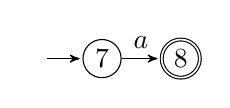
\begin{tikzpicture}[>=stealth',shorten >=1pt,auto,node distance=2cm,initial text=]
  \tikzset{every state/.style={inner sep=2pt,minimum size=0pt}}
  \node[initial,state]   (7) at (0, 0)  {7};
  \node[state,accepting] (8) at (1, 0)  {8};
  \path[->] (7)  edge node             {$a$} (8);
\end{tikzpicture}
\end{center}

\pause\smallskip

Using Rule 5, we get the NFA $N_{a*}$ for recognizing $a*$ as

\pause

\begin{center}
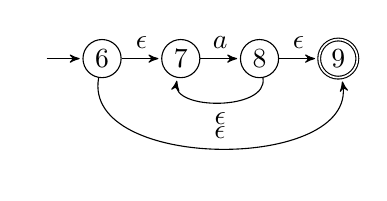
\begin{tikzpicture}[>=stealth',shorten >=1pt,auto,node distance=2cm,initial text=]
  \tikzset{every state/.style={inner sep=2pt,minimum size=0pt}}
  \node[initial,state] (6) at (0, 0)  {6};
  \node[state] (7) at (1, 0) {7};
  \node[state] (8) at (2, 0) {8};
  \node[state,accepting] (9) at (3, 0) {9};
  \path[->] (6)  edge node             {$\epsilon$} (7);
  \path[->] (7)  edge node             {$a$} (8);
  \path[->] (8)  edge [bend left=100] node {$\epsilon$} (7);
  \path[->] (6)  edge [bend right=100] node {$\epsilon$} (9);
  \path[->] (8)  edge node             {$\epsilon$} (9);  
\end{tikzpicture}
\end{center}

\pause\smallskip

Using Rule 3, we get the NFA $N_{(a|b)a*}$ for recognizing $(a|b)a*$

\pause

\begin{center}
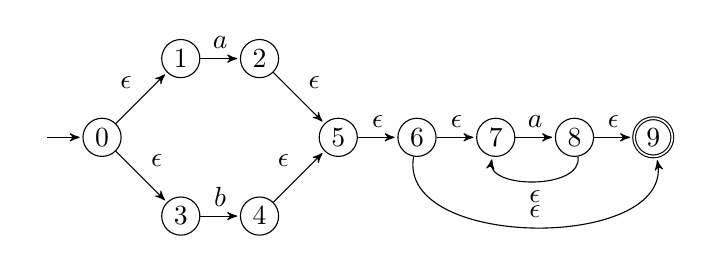
\begin{tikzpicture}[>=stealth',shorten >=1pt,auto,node distance=2cm,initial text=]
  \tikzset{every state/.style={inner sep=2pt,minimum size=0pt}}
  \node[initial,state] (0) at (0, 0)  {0};
  \node[state] (1) at (1, 1) {1};
  \node[state] (3) at (1, -1) {3};  
  \node[state] (2) at (2, 1) {2};
  \node[state] (4) at (2, -1) {4};  
  \node[state] (5) at (3, 0) {5};
  \node[state] (6) at (4, 0)  {6};
  \node[state] (7) at (5, 0) {7};
  \node[state] (8) at (6, 0) {8};
  \node[state,accepting] (9) at (7, 0) {9};
  \path[->] (0)  edge node             {$\epsilon$} (1);
  \path[->] (0)  edge node             {$\epsilon$} (3);
  \path[->] (1)  edge node             {$a$} (2); 
  \path[->] (3)  edge node             {$b$} (4); 
  \path[->] (2)  edge node             {$\epsilon$} (5);
  \path[->] (4)  edge node             {$\epsilon$} (5); 
  \path[->] (6)  edge node             {$\epsilon$} (7);
  \path[->] (7)  edge node             {$a$} (8);
  \path[->] (8)  edge [bend left=100] node {$\epsilon$} (7);
  \path[->] (6)  edge [bend right=100] node {$\epsilon$} (9);
  \path[->] (8)  edge node             {$\epsilon$} (9);  
  \path[->] (5)  edge node {$\epsilon$} (6);  
\end{tikzpicture}
\end{center}
\end{frame}

\begin{frame}[fragile]
\pause

Using Rule 2, we get the NFAs $N_b$ for recognizing the second instance of $b$ as

\pause

\begin{center}
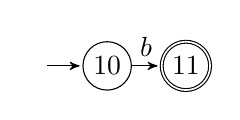
\begin{tikzpicture}[>=stealth',shorten >=1pt,auto,node distance=2cm,initial text=]
  \tikzset{every state/.style={inner sep=2pt,minimum size=0pt}}
  \node[initial,state]   (10) at (0, 0)  {10};
  \node[state,accepting] (11) at (1, 0)  {11};
  \path[->] (10)  edge node             {$b$} (11);
\end{tikzpicture}
\end{center}

\pause\smallskip

Finally, using Rule 3, we get the NFA $N_{(a|b)a*b}$ for recognizing $(a|b)a\!*\!b$ as

\pause

\begin{center}
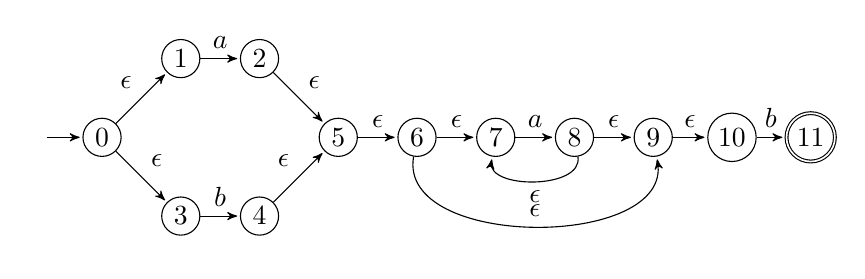
\begin{tikzpicture}[>=stealth',shorten >=1pt,auto,node distance=2cm,initial text=]
  \tikzset{every state/.style={inner sep=2pt,minimum size=0pt}}
  \node[initial,state] (0) at (0, 0)  {0};
  \node[state] (1) at (1, 1) {1};
  \node[state] (3) at (1, -1) {3};  
  \node[state] (2) at (2, 1) {2};
  \node[state] (4) at (2, -1) {4};  
  \node[state] (5) at (3, 0) {5};
  \node[state] (6) at (4, 0)  {6};
  \node[state] (7) at (5, 0) {7};
  \node[state] (8) at (6, 0) {8};
  \node[state] (9) at (7, 0) {9};
  \node[state] (10) at (8, 0) {10};  
  \node[state,accepting] (11) at (9, 0) {11};  
  \path[->] (0)  edge node             {$\epsilon$} (1);
  \path[->] (0)  edge node             {$\epsilon$} (3);
  \path[->] (1)  edge node             {$a$} (2); 
  \path[->] (3)  edge node             {$b$} (4); 
  \path[->] (2)  edge node             {$\epsilon$} (5);
  \path[->] (4)  edge node             {$\epsilon$} (5); 
  \path[->] (6)  edge node             {$\epsilon$} (7);
  \path[->] (7)  edge node             {$a$} (8);
  \path[->] (8)  edge [bend left=100] node {$\epsilon$} (7);
  \path[->] (6)  edge [bend right=100] node {$\epsilon$} (9);
  \path[->] (8)  edge node             {$\epsilon$} (9);  
  \path[->] (5)  edge node {$\epsilon$} (6);  
  \path[->] (9)  edge node             {$\epsilon$} (10);
  \path[->] (10)  edge node             {$b$} (11);  
\end{tikzpicture}
\end{center}
\end{frame}

\section{NFA to DFA}
\begin{frame}[fragile]
\pause

For any NFA, there is an equivalent DFA that can be constructed using the powerset (or subset) construction procedure

\pause\bigskip

The DFA is always in a state that simulates all the possible states that the NFA could possibly be in having scanned the same portion of the input

\pause\bigskip

The computation of all states reachable from a given state $s$ based on $\epsilon$-moves alone is called taking the $\epsilon$-closure of that state

\pause\bigskip

The $\epsilon$-closure$(s)$ for a state $s$ includes $s$ and all states reachable from $s$ using $\epsilon$-moves alone, ie, $\epsilon$-closure$(s) = \{s\} \cup \{r \in S | \text{ there is a path of only } \epsilon\text{-moves from } s \text{ to } r\}$

\pause\bigskip

The $\epsilon$-closure$(S)$ for a set of states $S$ includes $S$ and all states reachable from any state $s \in S$ using  $\epsilon$-moves alone
\end{frame}

\begin{frame}[fragile]
\pause

\begin{tcolorbox}[enhanced,drop shadow southwest,sharp corners,size=fbox,colback=white]
\begin{minipage}{\textwidth}
Algorithm: $\epsilon$-closure$(S)$ for a set of states $S$

\smallskip

Input: set of states $S$, set of moves $M$

\smallskip

Output: $\epsilon$-closure$(S)$
\end{minipage}
\end{tcolorbox}

\begin{overprint}
\onslide<2|handout:1>
\begin{tcolorbox}[enhanced,drop shadow southwest,sharp corners,size=fbox,colback=white,fontlower=\small\ttfamily,collower=silver900]

\begin{lstlisting}[language=Python,style=focusin]
def epsilonClosure(S, M):
    P = list(S)
    C = set(S)
    while len(P) != 0:
        r = P.pop()
        for s in M.m({r}, "epsilon"):
            if s not in C:
                P.append(s)
                C.add(s)
    return C
\end{lstlisting}

\tcblower
\begin{minipage}[t][.25cm][t]{\textwidth}

\end{minipage}
\end{tcolorbox}

\onslide<3|handout:2>
\begin{tcolorbox}[enhanced,drop shadow southwest,sharp corners,size=fbox,colback=white,fontlower=\small\ttfamily,collower=silver900]

\begin{lstlisting}[language=Python,style=focusout]
def epsilonClosure(S, M):
\end{lstlisting}
\begin{lstlisting}[language=Python,style=focusin,backgroundcolor=\color{lime100}]
    P = list(S)
\end{lstlisting}
\begin{lstlisting}[language=Python,style=focusout]
    C = set(S)
    while len(P) != 0:
        r = P.pop()
        for s in M.m({r}, "epsilon"):
            if s not in C:
                P.append(s)
                C.add(s)
    return C
\end{lstlisting}

\tcblower
\begin{minipage}[t][.25cm][t]{\textwidth}
stack containing all states in S
\end{minipage}
\end{tcolorbox}

\onslide<4|handout:3>
\begin{tcolorbox}[enhanced,drop shadow southwest,sharp corners,size=fbox,colback=white,fontlower=\small\ttfamily,collower=silver900]

\begin{lstlisting}[language=Python,style=focusout]
def epsilonClosure(S, M):
    P = list(S)
\end{lstlisting}
\begin{lstlisting}[language=Python,style=focusin,backgroundcolor=\color{lime100}]
    C = set(S)
\end{lstlisting}
\begin{lstlisting}[language=Python,style=focusout]
    while len(P) != 0:
        r = P.pop()
        for s in M.m({r}, "epsilon"):
            if s not in C:
                P.append(s)
                C.add(s)
    return C
\end{lstlisting}

\tcblower
\begin{minipage}[t][.25cm][t]{\textwidth}
closure initially contains states in S
\end{minipage}
\end{tcolorbox}

\onslide<5|handout:4>
\begin{tcolorbox}[enhanced,drop shadow southwest,sharp corners,size=fbox,colback=white,fontlower=\small\ttfamily,collower=silver900]

\begin{lstlisting}[language=Python,style=focusout]
def epsilonClosure(S, M):
    P = list(S)
    C = set(S)
\end{lstlisting}
\begin{lstlisting}[language=Python,style=focusin,backgroundcolor=\color{lime100}]
    while len(P) != 0:
\end{lstlisting}
\begin{lstlisting}[language=Python,style=focusout]
        r = P.pop()
        for s in M.m({r}, "epsilon"):
            if s not in C:
                P.append(s)
                C.add(s)
    return C
\end{lstlisting}

\tcblower
\begin{minipage}[t][.25cm][t]{\textwidth}
while P is not empty
\end{minipage}
\end{tcolorbox}

\onslide<6|handout:5>
\begin{tcolorbox}[enhanced,drop shadow southwest,sharp corners,size=fbox,colback=white,fontlower=\small\ttfamily,collower=silver900]

\begin{lstlisting}[language=Python,style=focusout]
def epsilonClosure(S, M):
    P = list(S)
    C = set(S)
    while len(P) != 0:
\end{lstlisting}
\begin{lstlisting}[language=Python,style=focusin,backgroundcolor=\color{lime100}]
        r = P.pop()
\end{lstlisting}
\begin{lstlisting}[language=Python,style=focusout]
        for s in M.m({r}, "epsilon"):
            if s not in C:
                P.append(s)
                C.add(s)
    return C
\end{lstlisting}

\tcblower
\begin{minipage}[t][.25cm][t]{\textwidth}
pop a state r off P
\end{minipage}
\end{tcolorbox}

\onslide<7|handout:6>
\begin{tcolorbox}[enhanced,drop shadow southwest,sharp corners,size=fbox,colback=white,fontlower=\small\ttfamily,collower=silver900]

\begin{lstlisting}[language=Python,style=focusout]
def epsilonClosure(S, M):
    P = list(S)
    C = set(S)
    while len(P) != 0:
        r = P.pop()
\end{lstlisting}
\begin{lstlisting}[language=Python,style=focusin,backgroundcolor=\color{lime100}]
        for s in M.m({r}, "epsilon"):
\end{lstlisting}
\begin{lstlisting}[language=Python,style=focusout]
            if s not in C:
                P.append(s)
                C.add(s)
    return C
\end{lstlisting}

\tcblower
\begin{minipage}[t][.25cm][t]{\textwidth}
for each state s reachable from r via an $\epsilon$-move
\end{minipage}
\end{tcolorbox}

\onslide<8|handout:7>
\begin{tcolorbox}[enhanced,drop shadow southwest,sharp corners,size=fbox,colback=white,fontlower=\small\ttfamily,collower=silver900]

\begin{lstlisting}[language=Python,style=focusout]
def epsilonClosure(S, M):
    P = list(S)
    C = set(S)
    while len(P) != 0:
        r = P.pop()
        for s in M.m({r}, "epsilon"):
\end{lstlisting}
\begin{lstlisting}[language=Python,style=focusin,backgroundcolor=\color{lime100}]
            if s not in C:
                P.append(s)
                C.add(s)
\end{lstlisting}
\begin{lstlisting}[language=Python,style=focusout]
    return C
\end{lstlisting}

\tcblower
\begin{minipage}[t][.25cm][t]{\textwidth}
add s to P and C if it is not in C
\end{minipage}
\end{tcolorbox}

\onslide<9|handout:8>
\begin{tcolorbox}[enhanced,drop shadow southwest,sharp corners,size=fbox,colback=white,fontlower=\small\ttfamily,collower=silver900]

\begin{lstlisting}[language=Python,style=focusout]
def epsilonClosure(S, M):
    P = list(S)
    C = set(S)
    while len(P) != 0:
        r = P.pop()
        for s in M.m({r}, "epsilon"):
            if s not in C:
                P.append(s)
                C.add(s)
\end{lstlisting}
\begin{lstlisting}[language=Python,style=focusin,backgroundcolor=\color{lime100}]
    return C
\end{lstlisting}

\tcblower
\begin{minipage}[t][.25cm][t]{\textwidth}
return C, the closure
\end{minipage}
\end{tcolorbox}
\end{overprint}
\end{frame}

\begin{frame}[fragile]
\pause

As an example, let's convert the NFA $N_{(a|b)a*b}$ to a DFA

\begin{center}
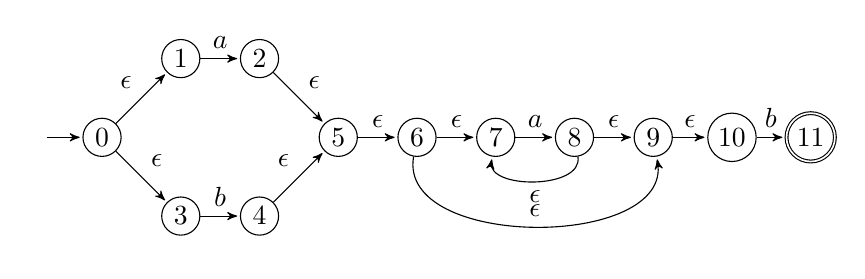
\begin{tikzpicture}[>=stealth',shorten >=1pt,auto,node distance=2cm,initial text=]
  \tikzset{every state/.style={inner sep=2pt,minimum size=0pt}}
  \node[initial,state] (0) at (0, 0)  {0};
  \node[state] (1) at (1, 1) {1};
  \node[state] (3) at (1, -1) {3};  
  \node[state] (2) at (2, 1) {2};
  \node[state] (4) at (2, -1) {4};  
  \node[state] (5) at (3, 0) {5};
  \node[state] (6) at (4, 0)  {6};
  \node[state] (7) at (5, 0) {7};
  \node[state] (8) at (6, 0) {8};
  \node[state] (9) at (7, 0) {9};
  \node[state] (10) at (8, 0) {10};  
  \node[state,accepting] (11) at (9, 0) {11};  
  \path[->] (0)  edge node             {$\epsilon$} (1);
  \path[->] (0)  edge node             {$\epsilon$} (3);
  \path[->] (1)  edge node             {$a$} (2); 
  \path[->] (3)  edge node             {$b$} (4); 
  \path[->] (2)  edge node             {$\epsilon$} (5);
  \path[->] (4)  edge node             {$\epsilon$} (5); 
  \path[->] (6)  edge node             {$\epsilon$} (7);
  \path[->] (7)  edge node             {$a$} (8);
  \path[->] (8)  edge [bend left=100] node {$\epsilon$} (7);
  \path[->] (6)  edge [bend right=100] node {$\epsilon$} (9);
  \path[->] (8)  edge node             {$\epsilon$} (9);  
  \path[->] (5)  edge node {$\epsilon$} (6);  
  \path[->] (9)  edge node             {$\epsilon$} (10);
  \path[->] (10)  edge node             {$b$} (11);  
\end{tikzpicture}
\end{center}

\pause\bigskip

\begin{overprint}
\onslide<3|handout:1>
\begin{center}
\begin{tabular}{|C{4cm}|C{.5cm}|C{4cm}|} \hline
$r$ & $a$ & $m(r, a)$ \\ \hline
\end{tabular}
\end{center}

\onslide<4|handout:2>
\begin{center}
\begin{tabular}{|C{4cm}|C{.5cm}|C{4cm}|} \hline
$r$ & $a$ & $m(r, a)$ \\ \hline \hline
$\epsilon\text{-closure}(0)$ & & \\ \hline
\end{tabular}
\end{center}

\onslide<5|handout:3>
\begin{center}
\begin{tabular}{|C{4cm}|C{.5cm}|C{4cm}|} \hline
$r$ & $a$ & $m(r, a)$ \\ \hline \hline
$\{0, 1, 3\} = 0$ (start state) & & \\ \hline
\end{tabular}
\end{center}

\onslide<6|handout:4>
\begin{center}
\begin{tabular}{|C{4cm}|C{.5cm}|C{4cm}|} \hline
$r$ & $a$ & $m(r, a)$ \\ \hline \hline
$\{0, 1, 3\} = 0$ (start state) & $a$ & \\ \hline
\end{tabular}
\end{center}

\onslide<7|handout:5>
\begin{center}
\begin{tabular}{|C{4cm}|C{.5cm}|C{4cm}|} \hline
$r$ & $a$ & $m(r, a)$ \\ \hline \hline
$\{0, 1, 3\} = 0$ (start state) & $a$ &  $\epsilon\text{-closure}(2)$ \\ \hline
\end{tabular}
\end{center}

\onslide<8|handout:6>
\begin{center}
\begin{tabular}{|C{4cm}|C{.5cm}|C{4cm}|} \hline
$r$ & $a$ & $m(r, a)$ \\ \hline \hline
$\{0, 1, 3\} = 0$ (start state) & $a$ &  $\{2, 5, 6, 7, 9, 10\} = 1$ \\ \hline
\end{tabular}
\end{center}

\onslide<9|handout:7>
\begin{center}
\begin{tabular}{|C{4cm}|C{.5cm}|C{4cm}|} \hline
$r$ & $a$ & $m(r, a)$ \\ \hline \hline
$\{0, 1, 3\} = 0$ (start state) & $a$ &  $\{2, 5, 6, 7, 9, 10\} = 1$ \\ \hline
$0$ & $b$ &   \\ \hline
\end{tabular}
\end{center}

\onslide<10|handout:8>
\begin{center}
\begin{tabular}{|C{4cm}|C{.5cm}|C{4cm}|} \hline
$r$ & $a$ & $m(r, a)$ \\ \hline \hline
$\{0, 1, 3\} = 0$ (start state) & $a$ &  $\{2, 5, 6, 7, 9, 10\} = 1$ \\ \hline
$0$ & $b$ & $\epsilon\text{-closure}(4)$  \\ \hline
\end{tabular}
\end{center}

\onslide<11|handout:9>
\begin{center}
\begin{tabular}{|C{4cm}|C{.5cm}|C{4cm}|} \hline
$r$ & $a$ & $m(r, a)$ \\ \hline \hline
$\{0, 1, 3\} = 0$ (start state) & $a$ &  $\{2, 5, 6, 7, 9, 10\} = 1$ \\ \hline
$0$ & $b$ & $\{4, 5, 6, 7, 9, 10\} = 2$  \\ \hline
\end{tabular}
\end{center}

\onslide<12|handout:10>
\begin{center}
\begin{tabular}{|C{4cm}|C{.5cm}|C{4cm}|} \hline
$r$ & $a$ & $m(r, a)$ \\ \hline \hline
$\{0, 1, 3\} = 0$ (start state) & $a$ &  $\{2, 5, 6, 7, 9, 10\} = 1$ \\ \hline
$0$ & $b$ & $\{4, 5, 6, 7, 9, 10\} = 2$  \\ \hline
$1$ & $a$ &   \\ \hline
\end{tabular}
\end{center}

\onslide<13|handout:11>
\begin{center}
\begin{tabular}{|C{4cm}|C{.5cm}|C{4cm}|} \hline
$r$ & $a$ & $m(r, a)$ \\ \hline \hline
$\{0, 1, 3\} = 0$ (start state) & $a$ &  $\{2, 5, 6, 7, 9, 10\} = 1$ \\ \hline
$0$ & $b$ & $\{4, 5, 6, 7, 9, 10\} = 2$  \\ \hline
$1$ & $a$ & $\epsilon\text{-closure}(8)$  \\ \hline
\end{tabular}
\end{center}

\onslide<14|handout:12>
\begin{center}
\begin{tabular}{|C{4cm}|C{.5cm}|C{4cm}|} \hline
$r$ & $a$ & $m(r, a)$ \\ \hline \hline
$\{0, 1, 3\} = 0$ (start state) & $a$ &  $\{2, 5, 6, 7, 9, 10\} = 1$ \\ \hline
$0$ & $b$ & $\{4, 5, 6, 7, 9, 10\} = 2$  \\ \hline
$1$ & $a$ & $\{7, 8, 9, 10\} = 3$  \\ \hline
\end{tabular}
\end{center}

\onslide<15|handout:13>
\begin{center}
\begin{tabular}{|C{4cm}|C{.5cm}|C{4cm}|} \hline
$r$ & $a$ & $m(r, a)$ \\ \hline \hline
$\{0, 1, 3\} = 0$ (start state) & $a$ &  $\{2, 5, 6, 7, 9, 10\} = 1$ \\ \hline
$0$ & $b$ & $\{4, 5, 6, 7, 9, 10\} = 2$  \\ \hline
$1$ & $a$ & $\{7, 8, 9, 10\} = 3$  \\ \hline
$1$ & $b$ &   \\ \hline
\end{tabular}
\end{center}

\onslide<16|handout:14>
\begin{center}
\begin{tabular}{|C{4cm}|C{.5cm}|C{4cm}|} \hline
$r$ & $a$ & $m(r, a)$ \\ \hline \hline
$\{0, 1, 3\} = 0$ (start state) & $a$ &  $\{2, 5, 6, 7, 9, 10\} = 1$ \\ \hline
$0$ & $b$ & $\{4, 5, 6, 7, 9, 10\} = 2$  \\ \hline
$1$ & $a$ & $\{7, 8, 9, 10\} = 3$  \\ \hline
$1$ & $b$ & $\epsilon\text{-closure}(11)$  \\ \hline
\end{tabular}
\end{center}

\onslide<17|handout:15>
\begin{center}
\begin{tabular}{|C{4cm}|C{.5cm}|C{4cm}|} \hline
$r$ & $a$ & $m(r, a)$ \\ \hline \hline
$\{0, 1, 3\} = 0$ (start state) & $a$ &  $\{2, 5, 6, 7, 9, 10\} = 1$ \\ \hline
$0$ & $b$ & $\{4, 5, 6, 7, 9, 10\} = 2$  \\ \hline
$1$ & $a$ & $\{7, 8, 9, 10\} = 3$  \\ \hline
$1$ & $b$ & $\{11\} = 4$ (accept state)  \\ \hline
\end{tabular}
\end{center}

\onslide<18|handout:16>
\begin{center}
\begin{tabular}{|C{4cm}|C{.5cm}|C{4cm}|} \hline
$r$ & $a$ & $m(r, a)$ \\ \hline \hline
$\{0, 1, 3\} = 0$ (start state) & $a$ &  $\{2, 5, 6, 7, 9, 10\} = 1$ \\ \hline
$0$ & $b$ & $\{4, 5, 6, 7, 9, 10\} = 2$  \\ \hline
$1$ & $a$ & $\{7, 8, 9, 10\} = 3$  \\ \hline
$1$ & $b$ & $\{11\} = 4$ (accept state)  \\ \hline
$2$ & $a$ &   \\ \hline
\end{tabular}
\end{center}

\onslide<19|handout:17>
\begin{center}
\begin{tabular}{|C{4cm}|C{.5cm}|C{4cm}|} \hline
$r$ & $a$ & $m(r, a)$ \\ \hline \hline
$\{0, 1, 3\} = 0$ (start state) & $a$ &  $\{2, 5, 6, 7, 9, 10\} = 1$ \\ \hline
$0$ & $b$ & $\{4, 5, 6, 7, 9, 10\} = 2$  \\ \hline
$1$ & $a$ & $\{7, 8, 9, 10\} = 3$  \\ \hline
$1$ & $b$ & $\{11\} = 4$ (accept state)  \\ \hline
$2$ & $a$ & $\epsilon\text{-closure}(8) = \{7, 8, 9, 10\}$ \\ \hline
\end{tabular}
\end{center}

\onslide<20|handout:18>
\begin{center}
\begin{tabular}{|C{4cm}|C{.5cm}|C{4cm}|} \hline
$r$ & $a$ & $m(r, a)$ \\ \hline \hline
$\{0, 1, 3\} = 0$ (start state) & $a$ &  $\{2, 5, 6, 7, 9, 10\} = 1$ \\ \hline
$0$ & $b$ & $\{4, 5, 6, 7, 9, 10\} = 2$  \\ \hline
$1$ & $a$ & $\{7, 8, 9, 10\} = 3$  \\ \hline
$1$ & $b$ & $\{11\} = 4$ (accept state) \\ \hline
$2$ & $a$ & $3$ \\ \hline
\end{tabular}
\end{center}

\onslide<21|handout:19>
\begin{center}
\begin{tabular}{|C{4cm}|C{.5cm}|C{4cm}|} \hline
$r$ & $a$ & $m(r, a)$ \\ \hline \hline
$\{0, 1, 3\} = 0$ (start state) & $a$ &  $\{2, 5, 6, 7, 9, 10\} = 1$ \\ \hline
$0$ & $b$ & $\{4, 5, 6, 7, 9, 10\} = 2$  \\ \hline
$1$ & $a$ & $\{7, 8, 9, 10\} = 3$  \\ \hline
$1$ & $b$ & $\{11\} = 4$ (accept state) \\ \hline
$2$ & $a$ & $3$ \\ \hline
$2$ & $b$ &  \\ \hline
\end{tabular}
\end{center}

\onslide<22|handout:20>
\begin{center}
\begin{tabular}{|C{4cm}|C{.5cm}|C{4cm}|} \hline
$r$ & $a$ & $m(r, a)$ \\ \hline \hline
$\{0, 1, 3\} = 0$ (start state) & $a$ &  $\{2, 5, 6, 7, 9, 10\} = 1$ \\ \hline
$0$ & $b$ & $\{4, 5, 6, 7, 9, 10\} = 2$  \\ \hline
$1$ & $a$ & $\{7, 8, 9, 10\} = 3$  \\ \hline
$1$ & $b$ & $\{11\} = 4$ (accept state) \\ \hline
$2$ & $a$ & $3$ \\ \hline
$2$ & $b$ &  $\epsilon\text{-closure}(11) = \{11\}$ \\ \hline
\end{tabular}
\end{center}

\onslide<23|handout:21>
\begin{center}
\begin{tabular}{|C{4cm}|C{.5cm}|C{4cm}|} \hline
$r$ & $a$ & $m(r, a)$ \\ \hline \hline
$\{0, 1, 3\} = 0$ (start state) & $a$ &  $\{2, 5, 6, 7, 9, 10\} = 1$ \\ \hline
$0$ & $b$ & $\{4, 5, 6, 7, 9, 10\} = 2$  \\ \hline
$1$ & $a$ & $\{7, 8, 9, 10\} = 3$  \\ \hline
$1$ & $b$ & $\{11\} = 4$ (accept state) \\ \hline
$2$ & $a$ & $3$ \\ \hline
$2$ & $b$ & $4$ \\ \hline
\end{tabular}
\end{center}

\onslide<24|handout:22>
\begin{center}
\begin{tabular}{|C{4cm}|C{.5cm}|C{4cm}|} \hline
$r$ & $a$ & $m(r, a)$ \\ \hline \hline
$\{0, 1, 3\} = 0$ (start state) & $a$ &  $\{2, 5, 6, 7, 9, 10\} = 1$ \\ \hline
$0$ & $b$ & $\{4, 5, 6, 7, 9, 10\} = 2$  \\ \hline
$1$ & $a$ & $\{7, 8, 9, 10\} = 3$  \\ \hline
$1$ & $b$ & $\{11\} = 4$ (accept state) \\ \hline
$2$ & $a$ & $3$ \\ \hline
$2$ & $b$ & $4$ \\ \hline
$3$ & $a$ &  \\ \hline
\end{tabular}
\end{center}

\onslide<25|handout:23>
\begin{center}
\begin{tabular}{|C{4cm}|C{.5cm}|C{4cm}|} \hline
$r$ & $a$ & $m(r, a)$ \\ \hline \hline
$\{0, 1, 3\} = 0$ (start state) & $a$ &  $\{2, 5, 6, 7, 9, 10\} = 1$ \\ \hline
$0$ & $b$ & $\{4, 5, 6, 7, 9, 10\} = 2$  \\ \hline
$1$ & $a$ & $\{7, 8, 9, 10\} = 3$  \\ \hline
$1$ & $b$ & $\{11\} = 4$ (accept state)  \\ \hline
$2$ & $a$ & $3$ \\ \hline
$2$ & $b$ & $4$ \\ \hline
$3$ & $a$ & $\epsilon\text{-closure}(8) = \{7, 8, 9, 10\}$ \\ \hline
\end{tabular}
\end{center}

\onslide<26|handout:24>
\begin{center}
\begin{tabular}{|C{4cm}|C{.5cm}|C{4cm}|} \hline
$r$ & $a$ & $m(r, a)$ \\ \hline \hline
$\{0, 1, 3\} = 0$ (start state) & $a$ &  $\{2, 5, 6, 7, 9, 10\} = 1$ \\ \hline
$0$ & $b$ & $\{4, 5, 6, 7, 9, 10\} = 2$  \\ \hline
$1$ & $a$ & $\{7, 8, 9, 10\} = 3$  \\ \hline
$1$ & $b$ & $\{11\} = 4$ (accept state)  \\ \hline
$2$ & $a$ & $3$ \\ \hline
$2$ & $b$ & $4$ \\ \hline
$3$ & $a$ & $3$ \\ \hline
\end{tabular}
\end{center}

\onslide<27|handout:25>
\begin{center}
\begin{tabular}{|C{4cm}|C{.5cm}|C{4cm}|} \hline
$r$ & $a$ & $m(r, a)$ \\ \hline \hline
$\{0, 1, 3\} = 0$ (start state) & $a$ &  $\{2, 5, 6, 7, 9, 10\} = 1$ \\ \hline
$0$ & $b$ & $\{4, 5, 6, 7, 9, 10\} = 2$  \\ \hline
$1$ & $a$ & $\{7, 8, 9, 10\} = 3$  \\ \hline
$1$ & $b$ & $\{11\} = 4$ (accept state) \\ \hline
$2$ & $a$ & $3$ \\ \hline
$2$ & $b$ & $4$ \\ \hline
$3$ & $a$ & $3$ \\ \hline
$3$ & $b$ &  \\ \hline
\end{tabular}
\end{center}

\onslide<28|handout:26>
\begin{center}
\begin{tabular}{|C{4cm}|C{.5cm}|C{4cm}|} \hline
$r$ & $a$ & $m(r, a)$ \\ \hline \hline
$\{0, 1, 3\} = 0$ (start state) & $a$ &  $\{2, 5, 6, 7, 9, 10\} = 1$ \\ \hline
$0$ & $b$ & $\{4, 5, 6, 7, 9, 10\} = 2$  \\ \hline
$1$ & $a$ & $\{7, 8, 9, 10\} = 3$  \\ \hline
$1$ & $b$ & $\{11\} = 4$ (accept state) \\ \hline
$2$ & $a$ & $3$ \\ \hline
$2$ & $b$ & $4$ \\ \hline
$3$ & $a$ & $3$ \\ \hline
$3$ & $b$ & $\epsilon\text{-closure}(11) = \{11\}$ \\ \hline
\end{tabular}
\end{center}

\onslide<29|handout:27>
\begin{center}
\begin{tabular}{|C{4cm}|C{.5cm}|C{4cm}|} \hline
$r$ & $a$ & $m(r, a)$ \\ \hline \hline
$\{0, 1, 3\} = 0$ (start state) & $a$ &  $\{2, 5, 6, 7, 9, 10\} = 1$ \\ \hline
$0$ & $b$ & $\{4, 5, 6, 7, 9, 10\} = 2$  \\ \hline
$1$ & $a$ & $\{7, 8, 9, 10\} = 3$  \\ \hline
$1$ & $b$ & $\{11\} = 4$ (accept state) \\ \hline
$2$ & $a$ & $3$ \\ \hline
$2$ & $b$ & $4$ \\ \hline
$3$ & $a$ & $3$ \\ \hline
$3$ & $b$ & $4$ \\ \hline
\end{tabular}
\end{center}
\end{overprint}
\end{frame}


\begin{frame}[fragile]
\pause
The DFA $D_{(a|b)a*b}$ for recognizing $(a|b)a\!*\!b$

\begin{center}
\tiny
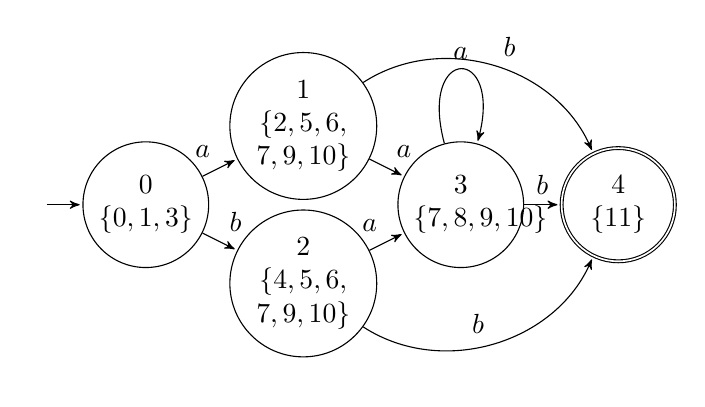
\begin{tikzpicture}[>=stealth',shorten >=1pt,auto,node distance=2cm,initial text=]
  \tikzset{every state/.style={inner sep=2pt,minimum size=0pt}}
  \node[initial,state] (0) at (0, 0)  {\parbox{1.2cm}{\centering $0$ \\ $\{0, 1, 3\}$}};
  \node[state] (1) at (2, 1)  {\parbox{1.2cm}{\centering $1$ \\ $\{2,5,6,$ \\ $7,9,10\}$}};
  \node[state] (2) at (2, -1)  {\parbox{1.2cm}{\centering $2$ \\ $\{4,5,6,$ \\ $7,9,10\}$}};  
  \node[state] (3) at (4, 0)  {\parbox{1.2cm}{\centering $3$ \\ $\{7,8,9,10\}$}};  
  \node[state,accepting] (4) at (6, 0)  {\parbox{1cm}{\centering $4$ \\ $\{11\}$}};   
  \path[->] (0)  edge node             {$a$} (1);
  \path[->] (0)  edge node             {$b$} (2);
  \path[->] (1)  edge node             {$a$} (3);
  \path[->] (2)  edge node             {$a$} (3);
  \path[->] (3)  edge node             {$b$} (4);
  \path[->] (1)  edge[bend right=-50] node             {$b$} (4);
  \path[->] (2)  edge[bend right=50] node             {$b$} (4);
  \path[->] (3)  edge[loop above] node             {$a$} (3); 
\end{tikzpicture}
\end{center}
\end{frame}

\begin{frame}[fragile]
\pause

\begin{algorithm}[H]
\begin{algorithmic}
\REQUIRE an NFA, $N = (\Sigma, S, s_0, M, F)$
\ENSURE DFA, $D = (\Sigma, S_D, s_{D0}, M_D, F_D)$
\STATE Set $s_{D0} \gets$  $\epsilon$-closure($s_0$)
\STATE Set $S_D$.add($s_{D0}$)
\STATE Moves $M_D$
\STATE Stack $stk$.push($s_{D0}$)
\STATE $i \gets 0$
\WHILE {!$stk$.empty()}
\STATE $t$ $\gets$ $stk$.pop()
\FOR {$a$ in $\Sigma$}
\STATE $s_{Di+1}$ $\gets$ $\epsilon$-closure($m(t, a)$)
\IF {$s_{Di+1} \neq \{\}$}
\IF {$s_{Di+1} \notin S_D$} 
\STATE $S_D$.add($s_{Di+1}$) \COMMENT{We have a new state}
\STATE $stk$.push($s_{Di+1}$)
\STATE $i \gets i + 1$
\STATE $M_D$.add($m_D(t,a) = i$)
\ELSIF {$\exists j, s_j \in S_D \text{ and } s_{Di+1} = s_j$} 
\STATE $M_D$.add($m_D(t, a) = j$) \COMMENT{In the case the state already exists}
\ENDIF
\ENDIF
\ENDFOR
\ENDWHILE
\end{algorithmic}
\caption{NFA to DFA Construction}
\end{algorithm}
\end{frame}

\begin{frame}[fragile]
\pause

\begin{algorithm}[H]
\begin{algorithmic}
\STATE Set $F_D$
\FOR {$s_D$ in $S_D$}
\FOR {$s$ in $s_D$}
\IF {$s \in F$}
\STATE $F_D$.add($s_D$)
\ENDIF
\ENDFOR
\ENDFOR
\RETURN $D = (\Sigma, S_D, s_{D0}, M_D, F_D)$
\end{algorithmic}
\caption{NFA to DFA Construction (contd.)}
\end{algorithm}
\end{frame}

\section{DFA to Minimal DFA}
\begin{frame}[fragile]
\pause

To obtain a smaller but equivalent DFA, we must combine states such that  the states in the new DFA are partitions of the states in the original (perhaps larger) DFA

\pause\bigskip

A good strategy is to start with just one or two partitions and then split them as necessary

\pause\bigskip

An obvious first partition has two sets: the set of final states and the set of non-final states
\end{frame}

\begin{frame}[fragile]
\pause

For example, consider the DFA for $(a|b)a*b$, partitioned as follows
\begin{center}
\visible<2->{\includegraphics[scale=0.6]{{figures/figure02.17}.jpg}}
\end{center}

\pause
\bigskip

The two states in this new DFA consist of the start state, $\{0, 1, 2, 3\}$ and the final state $\{4\}$ 

\pause
\bigskip

We must make sure that from a particular partition, each input symbol must move us to an identical partition
\end{frame}

\begin{frame}[fragile]
\pause

Beginning in any state in the partition $\{0, 1, 2, 3\}$, an $a$ takes us to one of the states in $\{0, 1, 2, 3\}$
\begin{align}
& m(0, a) = 1 \nonumber \\
& m(1, a) = 3 \nonumber \\
& m(2, a) = 3 \nonumber \\
& m(3, a) = 3 \nonumber
\end{align}

So, our partition $\{0, 1, 2, 3\}$ is fine so far as moves on the symbol $a$ are concerned

\pause
\bigskip

For the symbol $b$,
\begin{align}
& m(0, b) = 2 \nonumber \\
& m(1, b) = 4 \nonumber \\
& m(2, b) = 4 \nonumber \\
& m(3, b) = 4 \nonumber
\end{align}

So we must split the partition $\{0, 1, 2, 3\}$ into two new partitions, $\{0\}$ and $\{1, 2, 3\}$

\pause
\bigskip

If we are in state $s$, and for an input symbol $a$ in our alphabet there is no defined move $m(s, a) = t$, we invent a special dead state $d$, so that we can say $m(s, a) = d$
\end{frame}

\begin{frame}[fragile]
\pause

We are left with a partition into three sets: $\{0\}$, $\{1, 2, 3\}$ and $\{4\}$, as shown below

\begin{center}
\visible<2->{\includegraphics[scale=0.6]{{figures/figure02.18}.jpg}}
\end{center}
\end{frame}

\begin{frame}[fragile]
\pause

We need not worry about $\{0\}$ and $\{4\}$ as they contain just one state and so correspond to (those) states in the original machine

\pause
\bigskip

We consider $\{1, 2, 3\}$ to see if it is necessary to split it
\begin{align}
& m(1,a) = 3\nonumber \\
& m(2,a) = 3 \nonumber \\
& m(3, a) = 3 \nonumber
\end{align}
\begin{align}
& m(1, b) = 4 \nonumber \\
& m(2,b) = 4 \nonumber \\
& m(3, b) = 4 \nonumber
\end{align}

\pause
\bigskip

Thus, there is no further state splitting to be done, and we are left with the following smaller DFA

\begin{center}
\visible<4->{\includegraphics[scale=0.6]{{figures/figure02.19}.jpg}}
\end{center}
\end{frame}

\begin{frame}[fragile]
\pause

\begin{algorithm}[H]
\begin{algorithmic}
\REQUIRE a DFA, $D = (\Sigma, S, s_0, M, F)$
\ENSURE a partition of $S$
\STATE Set $partition \gets \{S - F, F\}$  \COMMENT{start with two sets: the non-final states and the final states} \\
\STATE{} \COMMENT {Splitting the states}
\WHILE {splitting occurs}
\FOR {Set $set$  in $partition$}
\IF {$set$.size() $>$ 1}
\FOR {Symbol $a$ in $\Sigma$}
\STATE{} \COMMENT{Determine if  moves from this `state' force a split}
\STATE State $s \gets$ a state chosen from $set$
\STATE $targetSet \gets$ the set in the partition containing $m(s, a)$
\STATE Set $set1 \gets \{\text{states } s \text{ from set } S, \text{ such that } m(s, a) \in targetSet\}$
\STATE Set $set2 \gets \{\text{states } s \text{ from set } S, \text{ such that } m(s, a) \notin targetSet\}$
\IF {$set2 \neq \{\}$}
\STATE{} \COMMENT{Yes, split the states.}
\STATE{replace $set$ in $partition$ by $set1$ and $set2$ and break out of the for-loop to continue with the next set in the partition}
\ENDIF
\ENDFOR
\ENDIF
\ENDFOR
\ENDWHILE
\end{algorithmic}
\caption{Minimizing a DFA}
\end{algorithm}
\end{frame}

\begin{frame}[fragile]
\pause

Let us run through another example, starting from a regular expression, producing an NFA, then a DFA, and finally a minimal DFA

\pause
\bigskip

Consider the regular expression $(a|b)*baa$ having the following syntactic structure

\begin{center}
\visible<3->{\includegraphics[scale=0.6]{{figures/figure02.20}.jpg}}
\end{center}
\end{frame}

\begin{frame}[fragile]
\pause

We apply the Thompson's construction procedure to produce the NFA shown below
\begin{center}
\visible<2->{\includegraphics[scale=0.6]{{figures/figure02.21}.jpg}}
\end{center}
\end{frame}

\begin{frame}[fragile]
\pause

Using the powerset construction method, we derive a DFA having the following states
\begin{align}
& s_0 = \{0, 1, 2, 4, 7, 8\} \nonumber \\
& m(s_0, a) : \{1, 2, 3, 4, 6, 7, 8\} = s_1 \nonumber \\
& m(s_0, b) : \{1, 2, 4, 5, 6,  7, 8, 9, 10\} = s_2 \nonumber \\
& m(s_1, a) : \{1, 2, 3, 4, 6, 7, 8\} = s_1 \nonumber \\
& m(s_1, b) : \{1, 2, 4, 5, 6, 7, 8, 9, 10\} = s_2 \nonumber \\
& m(s_2, a) : \{1, 2, 3, 4, 6, 7, 8, 11, 12\} = s_3 \nonumber \\
& m(s_2, b) : \{1, 2, 4, 5, 6, 7, 8, 9, 10\} = s_2 \nonumber \\
& m(s_3, a) : \{1, 2, 3, 4, 6, 7, 8, 13\} = s_4 \nonumber \\
& m(s_3, b) : \{1, 2, 4, 5, 6, 7, 8, 9, 10\} = s_2 \nonumber \\
& m(s_4, a) : \{1, 2, 3, 4, 6, 7, 8\} = s_1 \nonumber \\
& m(s_4, b) : \{1, 2, 4, 5, 6, 7, 8, 9, 10\} = s_2 \nonumber
\end{align}
\end{frame}

\begin{frame}[fragile]
\pause

The DFA itself is shown below
\begin{center}
\visible<2->{\includegraphics[scale=0.6]{{figures/figure02.22}.jpg}}
\end{center}
\end{frame}

\begin{frame}[fragile]
\pause

Finally, we use partitioning to produce the minimal DFA shown below
\begin{center}
\visible<2->{\includegraphics[scale=0.6]{{figures/figure02.23}.jpg}}
\end{center}
\end{frame}

\begin{frame}[fragile]
\pause

We re-number the states to produce the equivalent DFA shown below
\begin{center}
\visible<2->{\includegraphics[scale=0.6]{{figures/figure02.24}.jpg}}
\end{center}
\end{frame}

\section{JavaCC: a Tool for Generating Scanners}
\begin{frame}[fragile]
\pause

JavaCC (the CC stands for compiler-compiler) is a tool for generating lexical analyzers from regular expressions and parsers from context-free grammars

\pause
\bigskip

A lexical grammar specification consists a set of regular expressions and a set of lexical states; from any particular state, only certain regular expressions may be matched in scanning the input

\pause
\bigskip

There is a standard \lstinline{DEFAULT} state, in which scanning generally begins; one may specify additional states as required

\pause
\bigskip

Scanning a token proceeds by considering all regular expressions in the current state and choosing the one which consumes the greatest number of input characters

\pause
\bigskip

After a match, one can specify a state in which the scanner should go into; otherwise the scanner stays in the current state

\pause
\bigskip

There are four kinds of regular expressions, determining what happens when the regular expression has been matched
\begin{enumerate}
\item \lstinline{SKIP}: throws away the matched string
\item \lstinline{MORE}: continues to the next state, taking the matched string along
\item \lstinline{TOKEN}: creates a token from the matched string and returns it to the parser (or any caller)
\item \lstinline{SPECIAL_TOKEN}: creates a special token that does not participate in the parsing
\end{enumerate}
\end{frame}

\begin{frame}[fragile]
\pause

For example, a \lstinline{SKIP} can be used for ignoring white space
\begin{lstlisting}[language={}]
SKIP: {" "|"\t"|"\n"|"\r"|"\f"}
\end{lstlisting}

\pause
\bigskip

We can deal with single-line comments with the following regular expressions

\begin{lstlisting}
MORE: { "//": IN_SINGLE_LINE_COMMENT }
<IN_SINGLE_LINE_COMMENT>
SPECIAL_TOKEN: { <SINGLE_LINE_COMMENT: "\n"|"\r"|"\r\n" > : DEFAULT }
<IN_SINGLE_LINE_COMMENT>
MORE: { < ~[] > }
\end{lstlisting}

\pause
\bigskip

An alternative regular expression dealing with single-line comments

\begin{lstlisting}
SPECIAL_TOKEN: {
  <SINGLE_LINE_COMMENT: "//" (~["\n","\r"])* ("\n"|"\r"|"\r\n")>
}
\end{lstlisting}

\pause
\bigskip

Reserved words and symbols are specified by simply spelling them out; for example

\begin{lstlisting}
TOKEN: {
  < ABSTRACT: "abstract" >
| < BOOLEAN: "boolean" >
...

| < COMMA: "," >
| < DOT: "." >
}
\end{lstlisting}
\end{frame}

\begin{frame}[fragile]
\pause

A token for scanning identifiers

\begin{lstlisting}
TOKEN: {
  < IDENTIFIER: (<LETTER>|"_"|"$") (<LETTER>|<DIGIT>|"_"|"$")* >
| < #LETTER: ["a"-"z","A"-"Z"] >
| < #DIGIT: ["0"-"9"] >
}
\end{lstlisting}

\pause
\bigskip

A token for scanning literals

\begin{lstlisting}
TOKEN: {
  < INT_LITERAL: ("0" | <NON_ZERO_DIGIT> (<DIGIT>)*) >
| < #NON_ZERO_DIGIT: ["1"-"9"] >
| < CHAR_LITERAL: "'" (<ESC> | ~["'","\\","\n","\r"]) "'" >
| < STRING_LITERAL: "\"" (<ESC> | ~["\"","\\","\n","\r"])* "\"" >
| < #ESC: "\\" ["n","t","b","r","f","\\","'","\""] >
}
\end{lstlisting}

\pause
\bigskip

JavaCC takes a specification of the lexical syntax and produces several Java files, one of which is  \lstinline{TokenManager.java}, a program that implements a state machine; this is our scanner

\pause
\bigskip

The lexical specification for \jmm is contained in \lstinline{$j/j--/src/jminusminus/j--.jj}
\end{frame}
\end{document}
